\documentclass{tufte-handout}

%\geometry{showframe}
%\geometry{showframe}% for debugging purposes -- displays the margins

\usepackage{amsmath}
\usepackage{amssymb}
\usepackage{cleveref}
\crefname{Proposition}{Proposition}{Propositions}
\Crefname{Proposition}{Proposition}{Propositions}
\crefname{Theorem}{Theorem}{Theorems}
\Crefname{Theorem}{Theorem}{Theorems}
\crefname{Definition}{Definition}{Definitions}
\Crefname{Definition}{Definition}{Definitions}
\crefname{Corollary}{Corollary}{Corollaries}
\Crefname{Corollary}{Corollary}{Corollaries}
\crefname{Lemma}{Lemma}{Lemmas}
\Crefname{Lemma}{Lemma}{Lemmas}
\crefname{Example}{Example}{Examples}
\Crefname{Example}{Example}{Examples}
\usepackage{amsthm}

% Set up the images/graphics package
\usepackage{graphicx}
\setkeys{Gin}{width=\linewidth,totalheight=\textheight,keepaspectratio}
\graphicspath{{graphics/}}

% The following package makes prettier tables.  We're all about the bling!
\usepackage{booktabs}

% The units package provides nice, non-stacked fractions and better spacing
% for units.
\usepackage{units}

% The fancyvrb package lets us customize the formatting of verbatim
% environments.  We use a slightly smaller font.
\usepackage{fancyvrb}
\fvset{fontsize=\normalsize}

% Small sections of multiple columns
\usepackage{multicol}

% Provides paragraphs of dummy text
\usepackage{lipsum}

% Defines colors
\usepackage{xcolor}
\definecolor{blue}{cmyk}{0.63, 0.37, 0, 0.57}     
\definecolor{ltblue}{RGB}{78,150,179}

% These commands are used to pretty-print LaTeX commands
\newcommand{\doccmd}[1]{\texttt{\textbackslash#1}}% command name -- adds backslash automatically
\newcommand{\docopt}[1]{\ensuremath{\langle}\textrm{\textit{#1}}\ensuremath{\rangle}}% optional command argument
\newcommand{\docarg}[1]{\textrm{\textit{#1}}}% (required) command argument
\newenvironment{docspec}{\begin{quote}\noindent}{\end{quote}}% command specification environment
\newcommand{\docenv}[1]{\textsf{#1}}% environment name
\newcommand{\docpkg}[1]{\texttt{#1}}% package name
\newcommand{\doccls}[1]{\texttt{#1}}% document class name
\newcommand{\docclsopt}[1]{\texttt{#1}}% document class option name

% Package for title style
\usepackage{sectsty}
\usepackage[utf8]{inputenc}

% Sets section number style
\setcounter{secnumdepth}{3} % uncomment this, if desired
\renewcommand\thesection{\color{white}\arabic{section}}

% Sets title style
\makeatletter
  \renewcommand{\paragraph}{\@startsection{paragraph}%
    {4}{\z@}{-1ex \@plus -1ex \@minus -.3ex}%
    {0.5ex \@plus .2ex}{\normalfont\normalsize\bfseries}}
\makeatother

\makeatletter
  \renewcommand{\subsection}{\@startsection{subsection}%
    {3}{-1.8em}{-3ex \@plus -1ex \@minus -.2ex}%
    {1.5ex \@plus .2ex}
    {\hspace*{-5.5em}\fcolorbox{ltblue}{ltblue}{\parbox[c][1.0ex][b]{4em}{\phantom{space}}}
    \normalfont\large\itshape\color{ltblue}}}
\makeatother

\makeatletter
  \renewcommand{\section}{\@startsection{section}%
    {3}{-1.01em}{-3ex \@plus -1ex \@minus -.2ex}%
    {1.5ex \@plus .2ex}
    {\hspace*{-5.5em}\fcolorbox{blue}{blue}{\parbox[c][1.0ex][b]{4em}{\phantom{space}}}
    \normalfont\Large\itshape\color{blue}}}
\makeatother

% Sets theorem style
\usepackage{thmtools}
\usepackage{transparent}
\definecolor{theb}{rgb}{0.67, 0.80, 0.91}

\declaretheorem[shaded={bgcolor=Lavender,
    textwidth=30em}]{Definition} % Colorbox-styled Theorem 
\declaretheorem[shaded={bgcolor=Lavender,
    textwidth=30em}]{Theorem} % Colorbox-styled Theorem 
\declaretheorem[shaded={bgcolor=Thistle,
    textwidth=30em}]{Corollary} % Colorbox-styled Theorem
\declaretheorem[shaded={bgcolor=PeachPuff,
    textwidth=30em}]{Proposition} % Colorbox-styled Proposition
\declaretheorem[shaded={bgcolor=Thistle,
    textwidth=30em}]{Lemma} % Colorbox-styled Lemma
\declaretheorem[shaded={rulecolor=Lavender,
    rulewidth=2pt, bgcolor={rgb}{1,1,1}}]{Example-1} % Colorbounded-styled Theorem
\declaretheorem[thmbox=L]{boxtheorem L} % Theorem box L-size
\declaretheorem[thmbox=M]{Example} % Theorem box M-size
\declaretheorem[thmbox=S]{Formula} % Theorem box S-size
\declaretheorem[thmbox=S]{Statement} % Theorem box S-size

% set up pdf bookmark depth
\hypersetup{bookmarksdepth=3}

% ------------------------------------------------------------
\title{MATH240: Discrete Structures}
\author[Matthew He]{Matthew He}
\date{December 17, 2024} 
% if the \date{} command is left out, the current date will be used

% Beginning of the document
\begin{document}

\maketitle% this prints the handout title, author, and date

% abstract
\begin{abstract}
\noindent Abstract
\end{abstract}

% main text
\section{Foundation}
\subsection{Set Theory}
A set is a collection of distinct objects, called its elements or its members.

\paragraph{Set inclusion}
\begin{Proposition}
    The sets
    \[A = \{x \in \mathbb{Z}: \text{there exists } k \in \mathbb{Z} \text{such that } x = 2k + 1\}\]
    and
    \[B = \{x \in \mathbb{Z}: \text{there exists } k \in \mathbb{Z} \text{such that } x = 2l + 5\}\]
    are equal. (Both are different ways of describing the set of all odd integers.)
\end{Proposition}

\textit{Proof.} Let \( x \in A \). Then there exists \( k \in \mathbb{Z} \) such that \( x = 2k + 1 \).
Letting \( l = k - 2 \), we found that \( l \) is an integer. Furthermore,
\[ x = 2k + 1 = 2(k-2) + 5 = 2l + 5. \]
We have found \( l \) such that \( x = 2l + 5 \), so \( x \in B \). This shows that \( A \subseteq B \).

On the other hand, let \( x \in B \). Then there exists \( l \in \mathbb{Z} \) such that \( x = 2l + 5 \).
Now we let \( k = l + 2 \); \( k \in \mathbb{Z} \) since \( l \in \mathbb{Z} \). We have
\[ x = 2l + 5 = 2(l+2) + 1 = 2k + 1. \]
This shows that \( x \in A \), so \( B \subseteq A \). This combined with the previous
paragraph show \( A = B \). \qedsymbol

\paragraph{Set operations}
\begin{itemize}
    \item The \textit{union} of two sets \( A \) and \( B \), denoted by \( A \cup B \),
    is the set of all elements that are in \( A \) or in \( B \).
    \item The \textit{intersection} of two sets \( A \) and \( B \), denoted by \( A \cap B \),
    is the set of all elements that are in both \( A \) and \( B \).
    \item The \textit{difference} of two sets \( A \) and \( B \), denoted by \( A \backslash B \),
    is the set of all elements that are in \( A \) but not in \( B \).
    \item The \textit{symmetric difference} of two sets \( A \) and \( B \), denoted by \( A \triangle B \),
    is the set of all elements that are in exactly one of \( A \) and \( B \).
\end{itemize}

\subsection{Propositional Logic}
\textbf{Conditional and biconditional.}  The \textit{conditional}
logical relation IF q THEN p is denoted by \( p \Rightarrow q \).
\marginnote{The logical formula of these two conditionals are: \( p \Rightarrow q \equiv \neg p \vee q \) and \( q \Rightarrow p \equiv \neg q \vee p \).}
Within the conditional statement, p is called the \textit{antecedent}, which is the assumption.
The \textit{consequent} is q, which is the conclusion. The \textit{biconditional} logical relation
p IF AND ONLY IF q is denoted by \( p \Leftrightarrow q \). It asserts that variables p and q are logically equivalent.

\begin{table}
\centering
\begin{tabular}{c c c c}
\hline
$p$ & $q$ & $p \Rightarrow q$ & $p \Leftrightarrow q$ \\ \hline
1   & 1   & 1                 & 1                    \\ 
1   & 0   & 0                 & 0                    \\
0   & 1   & 1                 & 0                    \\ 
0   & 0   & 1                 & 1                    \\
\end{tabular}
\caption{Truth table for conditional and biconditional relations}
\end{table}

A formula is called a
\begin{itemize}
\item \textit{tautology} if it is true for all possible truth values of its variables.
\item \textit{contradiction} if it is false for all possible truth values of its variables.
\item \textit{contingency} if it is neither a tautology nor a contradiction.
\item \textit{satisfiable} if there is an assignment of truth values to its variables that makes it true.
\item \textit{falsifiable} if there is an assignment of truth values to its variables that makes it false.
\end{itemize}


\marginnote{\textbf{Tutorial}\\
\begin{enumerate}
    \item $ p \Rightarrow p $: tautology, since 
    $ \equiv \neg p \vee p = 1$ 
    \item $(p \Rightarrow q) \Rightarrow p$: contingency,
    true if $ p=q=1 $, false if $ p=0 $. \\
    (When $ p = 0 $, $ p \Rightarrow q  $is always true, and 
    a $ture \Rightarrow false (p)$ is always false.)
    \item $ (\neg (p \wedge \neg q)) \vee p \equiv 1 $: tautology. 
    \item $ (p \Leftrightarrow q) \wedge (p \Leftrightarrow \neg q )$: contradictory. 
\end{enumerate}
\begin{Example}
    Prove that a logical formula is satisfiable iff. its 
    negation is falsifiable.
\end{Example}
\textit{Proof.} A logical formula is satisfiable iff there is an assignment of 
all the variables which makes the formula true. By definition of the negation, this assignment makes the negation of our formula false, 
which means the negation is falsifiable. Proof of the converse is analogous.
}

\subsection{Predicate Logic}
    \begin{Definition}[Predicate]
    A \it predicate \rm is a statement containing some number
    of variable coming from a universe \textbf{u}. 
    \end{Definition}

\textbf{Negating quantifiers.} By De Morgan's laws, we have
\[\neg (\forall x \in U, P(x)) \equiv \exists x \in U, \neg P(x),\]
\[\neg (\exists x \in U, P(x)) \equiv \forall x \in U, \neg P(x).\]

Let's do some example. We express the statement, "There is a nonzero real numnber such that
every real number is not its inverse or is negative." In the universe \( \mathbb{R} \), ths formula corresponding
to the statement is
\[\exists x: (x\neq 0 \wedge (\forall y: xy \neq 1 \vee y < 0)).\]
If a formula is true then its negation is false. Let's deriv the negation of the formula above:
\begin{align*}
    \neg (\exists x: &(x\neq 0 \wedge (\forall y: xy \neq 1 \vee y < 0))) \\
    &\equiv \forall x: \neg (x\neq 0 \wedge (\forall y: xy \neq 1 \vee y < 0)) \\
    &\equiv \forall x: (x = 0 \vee \neg (\forall y: xy \neq 1 \vee y < 0)) \\
    &\equiv \forall x: (x = 0 \vee \exists y: \neg (xy \neq 1 \vee y < 0)) \\
    &\equiv \forall x: (x = 0 \vee \exists y: xy = 1 \wedge y \geq 0).
\end{align*}
Negating a formula in predicate logic is entirely mechanical. The \( \neg \) symbol
moves from left to right, flipping the quantifiers and negating the predicates as it goes.



\subsection{Proof Techniques}
\paragraph{Proofing statement of the form $ p \Rightarrow q $}
    We assume p is true, prove q, which is showing the case that p is true 
    be q is false can't happen.

    \begin{Proposition}
        If n is an odd integer, then $n^{2} $ is an odd integer.
    \end{Proposition}

    Write the proposition in predicate formula:
    \[u = \mathbb{Z }, \phantom{x} \forall n: ((\exists k : n = 2k+1) \Rightarrow (\exists n^{2} = 2l+1))\]
    \textit{proof.} Let n be ana integer. Assume that n is odd, that is, there exist k such that $ n = 2k+1 $.\\
    Then, $ n^{2} = (2k+1)^{2} = 2(2k^{2} + 2k) + 1 $. Let $ l = 2k^{2} + 2k $,
    then $ n^{2} = 2l + 1 $, thus, it's odd.

\paragraph{To disprove a statement: prove its negation is true}


\begin{Proposition}
    Disprove the statement: $\exists x \forall y: x + y \neq 0  $.
\end{Proposition}
\textit{Proof.}  
    To disprove, we shall prove its negation: $ \forall x \exists y : x+ y = 0 \equiv \neg (\exists x \forall y: x + y \neq 0) $
    Let $ x \in \mathbb{R } $ be given. Pick $ y = -x  $, then
$ x + y = 0 $. Q.E.D

\marginnote{Since $ p \wedge \neg p \equiv 0 $}

\paragraph{Converse and Contrapositive}

\begin{Definition}\phantom{x }\\
    \begin{enumerate}
        \item the \textbf{converse} of $ p \Rightarrow q  $ is $  q \Rightarrow p  $\\
        NB. $ p \Rightarrow q  \not\equiv  q \Rightarrow p  $
        \item the \textbf{contrapositive} of $ p \Rightarrow q  $ is$\neg q \Rightarrow \neg p  $ \\
        $ p \Rightarrow q  \equiv \neg p \vee q \equiv \neg q \Rightarrow \neg p$
    \end{enumerate}
\end{Definition}

\paragraph{Proofs by contradiction}
You assume something is true, and get something nonsense.\\
\[\neg p \Rightarrow 0 \equiv \neg (\neg p) \vee 0 \equiv p\]

\begin{Proposition}
    There is no least positive rational number.\\
    \[u = \mathbb{Q }: \neg (\exists x : x>0 \wedge (\forall y: y > 0 \Rightarrow x \leq y))\]
\end{Proposition}

\textit{Proof.} Suppose, for a contradiction that the proposition is false, that is,
there exist $  x \in \mathbb{ Q } $ such that $ x>0 $ and for all $ y \in \mathbb{Q } $ with $ y>0, x \leq y  $.\\
Let $ y = \frac{x }{2}$, we have $ \frac{x }{2} > 0 $ since $ x>0 $. Then $ x \leq y  $, so $ x \leq \frac{x }{2} $.\\
Divide through by x ( because x > 0) to get $ 1 \leq \frac{1}{2}$.\\
the contradiction completes the proof. Q.E.D

\marginnote{\textbf{Tutorial: Prove or disprove:}\\
\begin{enumerate}
  \item $ \forall n \in \mathbb{N }, \exists m \in \mathbb{N }, n + m = 0 $ \\
  False. Let's proof its negation: $ \exists n \in \mathbb{N }, \forall m \in \mathbb{N },
  n + m \neq 0$, it's true, e.g., we can let $ n = 2 $.
  \item $ \forall n \in \mathbb{N }, \exists m \in \mathbb{Z }, n + m = 0 $\\
  Ture, Let $ n \in \mathbb{N } $, then choose $ m = -n \in \mathbb{Z }  $, and we get $ m+n=0 $. 
  \item $ \forall n \in \mathbb{N }, \exists k \in \mathbb{N }, (k \geq m) \Rightarrow (k \geq 5n) $: \\
  The statement is equivalent to $ (k < m) \vee (k \geq 5n)$. \\
  For any $ n \in \mathbb{N }$, choose $m = 5n $, then for all $ k \in \mathbb{N } $, we have that statement is true.
\end{enumerate}}


\paragraph{Case Analysis}

\begin{Proposition}
    \textit{prop.} There exists irrational numbers a,b such that \( a^b \) is rational.
\end{Proposition}


\subsection{Functions}
\begin{Definition}[Surjective and injective]
    A function is surjective if 
    \[\forall b \in B, \exists a \in A, f(a) = b\]
    A function is injective if 
    \[\forall a_1, a_2 \in A, a_1 \neq a_2 \rightarrow f(a_1) \neq f(a_2)\]
    or $  f(a_1) = f(a_2)  \rightarrow a_1 = a_2$.
\end{Definition}

\begin{Theorem}
    Let \( a_1,a_2,\ldots,a_n \) be a finite sequence (repeats allowed) of real numbers. Let
    \[a = \frac{1}{n} \sum_{i=1}^{n} a_i.\]
    be the average value of the sequence and let \( m \) 
    be the maximum value of the sequence attains. Then \( m \geq a \).
\end{Theorem}

\begin{Theorem}
    Let A and B be finite sets with \( \left|A\right| = m\) and \( \left|B\right| = n \).
    For every function \( f:A \to B \), then there is some \( b \in B \) such that
    there are at least \( \lceil m/n \rceil \) elements in \( A \) that get mapped to \( b \).
\end{Theorem}

\begin{Corollary}[The pigeonhole principle]
    Let \( n \geq 2 \). If \( n \) pigeons nest in \( n-1 \) holes, there is at least one hole that contains at least two pigeons.
    Let \( f:A \to B \) be a function. 
    If \( \left|A\right| > \left|B\right| \), then \( f \) is not injective.
\end{Corollary}

\textbf{Bijections.} A function is called \textit{bijective} if it is both surjective and injective.

\begin{Proposition}
    Let A and B be finite sets. Then
    \begin{enumerate}
        \item there exists a bijection \( f:A\to B \) if and only if \( \left|A\right| = \left|B\right| \); and
        \item if \(\left|A\right| = \left|B\right| \), \( f:A\to B \) then \( f \) is injective if and only if \( f \) is surjective.
    \end{enumerate}
\end{Proposition}

\textbf{Invertibility.} A function \( f:A\to B \) is called \textit{invertible} if there exists a function \( g:B\to A \) such that
\begin{enumerate}
    \item for all \( a \in A \), \( g(f(a)) = a \); and
    \item for all \( b \in B \), \( f(g(b)) = b \).
\end{enumerate}
If such a function \( g \) exists, it is unique, and we call it the \textit{inverse} of \( f \), denoted by \( f^{-1} \).

\begin{Proposition}
    Let \( f:A\to B \) be a function. Then \( f \) is invertible if and only if
    \( f  \) is bijective.
\end{Proposition}

\textit{Proof.} First we assume that \( f \) is invertible. So there exists an inverse \( g  \) of \( f  \).
For each \( b \in B  \), setting \( a = g(b ) \) we have 
\[ f(a) = f(g(b)) = b. \]
This prove that \( f \) is surjective. To show that \( f \) is injective, suppose that \( f(a_1) = f(a_2) \).
By applying \( g \) to both sides, we get \(g(f(a_1)) = g(f(a_2)) \), whence \( a_1 = a_2 \), by definition of \( g \).

Noew assume that \( f \) is bijective. We shall construct an inverse \( g \) of \( f \). Given any \( b \in B \),
there is some \( a \in A \) such that \( f(a) = b \), from surjectivity of \( f \), and
this \( a \) is unique, by injectivity of \( f \). So set \( g(b) = a \) (and repeat this process for
every \( b \in B \)). We have \( f(g(b)) = f(a) = b \), and for every \( a \in A \), by definition of \( g \)
the element \( g(f(a)) \) is the unique element in \( A \) that gets brought to \( f(a) \) by \( f \), so
has to be \( a \) itself. \hfill \qedsymbol

Sometimes to prove that two sets have the same cardinality, it is easier to prove that there exists
a bijection between them. Here is an example:
\begin{Proposition}
    \label{prop:even_odd_cardinality}
    Let X be a finite nonempty set. Let E be the set of all subsets of X with even cardinality, and
    let D be the set of all subsets of X with odd cardinality. Then \( \left|E\right| = \left|D\right| \).
\end{Proposition}

\subsection{Cardinality}
We say that A and B are \textit{equipotent} or have the same \textit{cardinality}, 
if and only if there exists a bijection \( f:A\to B \). We write \( \left|A\right| = \left|B\right| \).

\marginnote{It is possible to remove an infinite number of elements from \( \mathbb{N} \) and end up with something 
still equipotent with \( \mathbb{N} \).}

\begin{Theorem}
    We have \( \left|N\right| = \left|Z \right| \).
\end{Theorem}

We say that a set A is countably infinite if if there exists a bijection \( f:N\to A \), that is
if \( \left|N\right| = \left|A\right| \). A set is countable if it is finite or countably infinite.
Otherwise it is called uncountable.

Sometimes it is difficult to come up with a bijection between two sets. Instead,
we would like to find an injection from B to A.

\begin{Theorem}[Schroder-Bernstein Theorem]
    If there exists an injective function \( f:A\to B \) and another injective function \( g:B\to A \),
    then there exists a bijection \( h:A\to B \).
\end{Theorem}

\begin{Theorem}[Fundamental Theorem of Arithmetic]
Every positive integer \( n \geq 2 \) can be factored into a product
\[
n = p_1^{v_1} p_2^{v_2} \cdots p_k^{v_k},
\]
where the \( p_i \) are distinct prime numbers and the \( v_i \) are positive integers.
 This factorization is unique up to the order of the factors; 
 that is, apart from the sequence in which the primes appear, there is
  only one way to factor \( n \) into primes.
\end{Theorem}
    
\begin{Theorem}
    If A and B are countably infinite sets, then \( A \times B\) is also
    countably infinite.
\end{Theorem}

\begin{Corollary}
    We have \( \left| \mathbb{Z} \times \mathbb{Z} \right| = \left| \mathbb{N} \right| \).
\end{Corollary}

\begin{Theorem}
    The set \( \mathbb{Q} \) of rational numbers is countable.
\end{Theorem}

\begin{Theorem}
    The set A of all infinite binary sequences is uncountable.
\end{Theorem}

\subsection{Relations}
\begin{Definition}
A \textit{relation} on a set X is a subset \( R \subseteq X \times X \).
If \( (a,b) \in R \), we write \( aRb \) and say that a is related to b.
\end{Definition}

\textbf{Properties of relations.} Let R be a relation on a set X. We say that R is
\begin{enumerate}
    \item \textit{reflexive} if \( aRa \) for all \( a \in X \).
    \item \textit{symmetric} if \( aRb \) implies \( bRa \) for all \( a,b \in X \).
    \item \textit{transitive} if \( aRb \) and \( bRc \) implies \( aRc \) for all \( a,b,c \in X \).
\end{enumerate}

\begin{Definition}[Equivalence relations]
    If R is reflexive, symmetric, and transitive, we say that R is an \textit{equivalence relation}.
\end{Definition}
If R is an equivalence relation, often we shall write \( a \sim b \) to mean \( aRb \).
Sometimes we might even just say that \( \sim \) is the equivalence relation.
\begin{Definition}[Equivalence class]
    Let \(R \subseteq X \times X \) be an equivalence relation on a set X. Define the \textit{equivalence class} of an element \( a \in X \) to
    be the set
    \[ [a] = \{b \in X: a\sim b\}. \]
\end{Definition}

\begin{Proposition}
    Let R be an equivalence relation on A. Then
    \begin{enumerate}
        \item for all \( x \in A \), \( x \in [x] \);
        \item for all \( x,y \in A \), \( x\sim y \) if and only if \( [x] = [y] \);
        \item for all \( x,y \in A \), \( x \not\sim y \) if and only if \( [x] \cap [y] = \emptyset \).
    \end{enumerate}
\end{Proposition}

\begin{Definition}[Quotient set]
    Let A be a set and let \( \sim \) to be an equivalence relation on A.
    We define the \textit{quotient} of A by \( \sim \) as the set of all equivalence classes of A under \( \sim \):
    \[ A\slash \sim = \{[x]: x \in A\}. \]
\end{Definition}

\begin{Proposition}
    Let A be a set and let \( \sim \) to be an equivalence relation on A. 
    Then \(A\slash \sim\) is a partition of A.
\end{Proposition}

\section{Number Theory}
\subsection{Division}

\begin{Proposition}
    For all \( a,b,c \in \mathbb{Z} \),
    \begin{enumerate}
        \item if \( a|b \) then \( a|bc \);
        \item if \( a|b \) and \( a|c \) then \( a|(b+c) \);
        \item if \( a|b \) and \( b|c \) then \( a|c \);
        \item if \( a|b \) and \( b\neq 0 \), then \( |a| \leq |b| \); and
        \item if \( a|b \) and \( b|a \), then \( \left|a\right| = \left|b\right|\).
    \end{enumerate}
\end{Proposition}

\begin{Theorem}[Division algorithm]
    Let \( a , b \in \mathbb{Z} \) with \( b > 0 \). Then there exist unique integers \( q,r \in \mathbb{Z} \) such that
    \[ a = bq + r \text{ and } 0 \leq r < \left|b\right|.\]
\end{Theorem}

\textbf{Euclid's algorithm.} 
Given two nonnegative integers \( a \) and \( b \), not both zero, this algorithm outputs \( \gcd(a,b) \).
\begin{enumerate}
    \item[E1.] If \( b = 0 \), output \( a \) and stop.
    \item[E2.] Since \( b\neq 0 \), by the division algorithm we may write \( a = bq + r \) with \( 0 \leq r < b \).
    Set \( a \leftarrow b \) and \( b \leftarrow r \), and return to step E1.
\end{enumerate}
Why does this algorithm work? The following lemma clarifies the situation.
\begin{Lemma}
    Let \( a,b,q,r \in \mathbb{Z} \) be integers such that \( a = bq + r \).
    Then \( \gcd(a,b) = \gcd(b,r) \).
\end{Lemma}

\begin{Theorem}[Bezout's identity]
    Let \( a,b \in \mathbb{Z} \) be nonzero integers with greatest common divisor \( \gcd(a,b) \). 
    Then there exist integers \( s,t \) such that
    \[ \gcd(a,b) = sa + tb. \]
    Moreover, \( \gcd(a,b) \) is the smallest positive integer that can be written in an
    integer linear combination of \( a \) and \( b \).
\end{Theorem}

\marginnote{The proof of Bezout's identity is a good example of a minimality proof.}


\begin{Proposition}
    Let a and b be nonzero integers. The set
    \[X = \left\{s'a+t'b:s',t'\in \mathbb{Z}\right\}\]
    is exactly the set of multiples of $ d = \gcd(a,b) $.
\end{Proposition}
\textit{Proof.} By Bezout's identity, there exist integers $ s,t $ such that \( d = sa+tb \).
First let \( n \in \mathbb{Z} \) be a multiple of \( d \), so \( n = kd \) for some \( k \in \mathbb{Z} \).
Then we have \[n=kd=d(sa+tb)=(ds)a+(dt)b,\]
which means that \( n\in \mathbf{X} \), since \( ds,dt \in \mathbb{Z} \).

Conversely, suppose that \( n \in \mathbf{X} \). Then \( n = s'a+t'b \) for some \( s',t' \in \mathbb{Z} \).
Then since \( d \) divides \( a \) and \( b \), we can write \( a=ld \) and \( b=md \) for some integers \( l,m \in \mathbb{Z}\).
So we have \[n=s'a+t'b=s'ld+t'md=(s'l+t'm)d,\]
which shows that \( d|n \), since \( s'l+t'm \in \mathbb{Z} \). \qedsymbol

\textbf{Coprime} We say that integers \( a \) and \( b \) are relatively prime or coprime if \( \gcd(a,b) = 1 \).

\begin{Proposition}
    For all integers \( n>1 \), \( n \) and \( n+1 \) are relatively prime.
\end{Proposition}

\subsection{Primes}
\begin{Theorem}
    An integer \( p \) with \( p\geq 2 \) is prime if and only if the only if for
    all \( a,b \in \mathbb{N} \), \( p|ab \) implies that \( p|a \) or \( p|b \).
\end{Theorem}

\marginnote{This relates to the definition of a prime number as a number \( p \) such that \( \gcd(p, n) = 1 \) for
 all integers \( n \) with \( 1 < n < p \). 
 Since \( p \) shares no common divisors with any number less than 
 itself (other than 1), it cannot divide a product \( ab \) unless 
 it divides at least one of \( a \) or \( b \). 
 This emphasizes the fundamental property of prime numbers in relation to 
 divisibility and greatest common divisors.}

To illustrate that this theorem, we can also consider \( p=6,a=2 \) and \( b=15 \).
We have \( p|ab \) since \( 6|30 \), but \( 6 \) does not divide \( 2 \) or \( 15 \).\\

By induction, the theorem can be extended to arbitrary finite products.
\begin{Corollary}
    Let \( p \) be prime and \( n \) be a positive integer. If \( a_1, a_2, \ldots,a_n \) are
    integers such that \( p|a_1a_2\cdots a_n \), then \( p|a_i \) for some \( 1\leq i \leq n \).
\end{Corollary}

\begin{Theorem}[Fundamental Theorem of Arithmetic, again]
    Every integer \( n \geq 2 \) can be expressedc as a product
    \[ n = p_1p_2\cdots p_k \]
    where \( p_1\leq p_2\leq \cdots \leq p_k \) are prime numbers.
    Furthermore, this factorization is unique.
\end{Theorem}

The Fundamental Theorem of Arithmetic can be used to prove the following theorem.
\begin{Theorem}
    Let \( k \) and \( n \) be positive integers. Then either \( \sqrt[k]{n} \) is an integer or
    it is irrational.
\end{Theorem}

\begin{Theorem}
    There are infinitely many prime numbers.
\end{Theorem}

Although the set of prime numbers is infinite, it does sort of get "sparser" as one heads off towards infinity.
This is quantified by the following theorem.

\begin{Theorem}[Prime number theorem]
    For \( x \in \mathbb{R} \), let 
    \[ \pi(x) = \left|\left\{ p \leq x : p \text{ is prime}\right\}\right|.\]
    Then \( \pi(x) \sim x \slash \ln x \) in the sense that
    \[ \lim_{x\to \infty} \frac{\pi(x)}{x/\ln x} = 1. \]
    
\end{Theorem}


\begin{Corollary}
    Let \( n \) be a positive integer and let \( m \) be chosen uniformly at random from the set \( \{1,2,\ldots,n\} \).
    Then the probability that \( m \) is primes satisfies
    \[(\ln n ) \mathbb{P}\{m\text{ prime}\} \to 1\]
    as \( n \to \infty \). In other word, the probability that that \( m \) is prime is 
    asymptotically \( 1/\ln n \).
\end{Corollary}

\subsection{Modular Arithmetic}

\begin{Definition}[Congruence]
    Fix \( n \geq 1 \) and let \( a,b \in \mathbb{Z} \). We say that \( a \) is congruent to \( b \) modulo \( n \),
    if \( n|a-b \). i.e., if \( a-b = kn\)  for some \( k \in \mathbb{Z} \). We write this as \( a \equiv_n b \)
    or \( a \equiv b \pmod{n} \).
\end{Definition}

For any fixed \( n \), the set of all \( (a,b)\in \mathbb{Z} \) with \( a \equiv_n b \)  is a relation on \( \mathbb{Z} \).

\begin{Proposition}
    For all fixed \( n \), the relation \( a \equiv_n b\) is an equivalence relation on the set \( \mathbb{Z} \).
\end{Proposition}

\begin{Proposition}
    Fix an integer \( n \geq 2 \). Let \( a,b\in \mathbb{Z} \). Then \( a \equiv_n b \) if and only if
    \[a \text{ \% } n = b \text{ \% } n.\]
\end{Proposition}

This proposition is useful in practice if we want to know whether two numbers are congruent modulo \( n \).

The proposition also implies that for all \( a \in \mathbb{Z} \) and \( n \geq 2 \),
one has \( [a]_n = [a \text{ \% } n] \). 
From the division algorithm, we know that \( a \text{ \% } n \) is an element in the \( [0,n) \).
It is equal to the integer \( r \) in that range such that we may write \( a = qn + r \) for some \( q \in \mathbb{Z} \).
We may choose to denote the whole equivalence class by this element \( r \). The set
\[ \mathbb{Z}\slash n\mathbb{Z} = \mathbb{Z} \slash \equiv_n = \{[0],[1],\ldots,[n-1]\} \]
is called the \textit{ring of integers modulo n}. or the \textit{cyclic group on n elements}.

\paragraph{Computation in modular arithmetic}
An element \( a\in \mathbb{Z} \) with \( a \not\equiv_n 0 \) is said to be a zero divisor if there exists 
\( b\in \mathbb{Z} \) with \( b \not\equiv_n 0 \) such that \( ab \equiv_n 0 \).

\begin{Proposition}
    Let \( a\equiv_n c  \) and \( b\equiv_n d \). Then
    \begin{enumerate}
        \item \( a+b \equiv_n c+d \);
        \item \( ab \equiv_n cd \);
        \item \( a^k \equiv_n c^k \) for all \( k \in \mathbb{N} \);
    \end{enumerate}
\end{Proposition}

\begin{Definition}[Inverses modulo n]
    An element \( a \in \mathbb{Z} \) is said to be invertible modulo \( n \) if there exists \( b \in \mathbb{Z} \) such that
    \( ab \equiv_n 1 \). The element \( b \) is called the \textit{inverse} of a.
    In fact, inverses are unique (in \( \mathbb{Z} \slash n \mathbb{Z} \))
\end{Definition}

\begin{Proposition}
    Let \( a,n \in \mathbb{Z}\) with \( n \geq 2 \). Then if \( ab \equiv_n 1 \), and
    \( ac \equiv_n 1 \), then \( b \equiv_n c \).
\end{Proposition}

\begin{Theorem}
    Let \( a,n \in \mathbb{Z} \) with \( n \geq 2 \). Then:
    \begin{enumerate}
        \item \( a \) is invertible modulo \( n \) if and only if \( \gcd(a,n) = 1 \);
        \item if \( a \) is invertible modulo \( n \), then there is a unique \( b \in \mathbb{Z} \) such that
        \( ab \equiv_n 1 \). Namely, if 
        \[ 1 = sa + tn ,\]
        then we can set \( b = s \text{ \% } n\).
    \end{enumerate}
\end{Theorem}

We can use this theorem to systematically find inverses of integers modulo other integers.

\begin{Proposition}
    Let \( p \) be prime. Then
    \begin{enumerate}
        \item every \( x\in \mathbb{Z} \) with \( x \not\equiv_p 0 \) is invertible modulo \( p \);
        \item for all \( a,b \in \mathbb{Z} \) with \( ab\equiv_p 0 \) one has \( a \equiv_p 0 \) or \( b \equiv_p 0 \).
    \end{enumerate}
\end{Proposition}

\paragraph{Solving congruences modulo n}

\begin{Proposition}
    Let \( p \) be prime. Then \( a^2 \equiv a \pmod{p} \) if and only if \( a \) is either
    congruent to 0 or 1 modulo \( p \).
\end{Proposition}

\begin{Proposition}
    Let \( p \) be prime and let \( a \not\equiv 0 \pmod{p} \) (so that \( a \) is invertible modulo \( p \)).
    Then \( a \equiv a^{-1} \pmod{p} \) if and only if \( a \) is either congruent to 1 or \( -1 \) modulo \( p \).
\end{Proposition}

\begin{Theorem}[Fermat's little theorem]
    Let \( p \) be prime and let \( a \) be an integer. If \( a \not\equiv-p 0 \), then
    \[ a^{p-1} \equiv 1 \pmod{p}. \]
\end{Theorem}

\begin{Lemma}
    For all prime number \( p \), the integer \( (p-1)!\) is congruent to \( -1 \) modulo \( p \).
\end{Lemma}

\begin{Theorem}[Wilson's theorem]
    For all integers \( n \geq 2 \), the integer \( n \) is prime if and only if
    \[ (n-1)! \equiv -1 \pmod{n}. \]
\end{Theorem}

\section{Graph Theory}
\subsection{Definitions}
A graph is a pair $ G = (V,E) $, where V is a nonempty set and \[E \subseteq \left\{ {u,v}: u,v \in V, u \neq v\right\}.\]

\marginnote{The graph \( G \) is said to be \textit{finite} if both \( V \) are finite sets.
A simple graph is a graph that does not have more than one edge between any two vertices and no edge
starts and ends at the same vertex.}

\textbf{Degrees and k-regularity}
The \textit{neighbors} of a vertex \( v \) are all \( u \in V \) such that \( uv \in E \). The 
\textit{degree} of a vertex \( v \) is the number of neighbors of \( v \), denoted by \( deg(v) \).
A graph is said to be \( k-regular \) for some \( k\in \mathbb{N} \) if every \( v \in V \) has degree \( k \).

The following theorem relates vertex degree to the number of edges.
\begin{Theorem}
    Let G = (V,E) be a finite graph. Then \[\sum_{v \in V} \deg(v) = 2 \left|E\right|.\]
\end{Theorem}

\begin{Corollary}[Handshaking Lemma]
    In every finite simple graph, the number of vertices having odd degree is even.
\end{Corollary}

From Theorem above, we can derive a corollary that counts the number of edges in k-regular graphs.

\begin{Corollary}
    Let G = (V,E) be k-regular. Then \[\left|E\right| = \frac{k\left|V\right|}{2}.\]
\end{Corollary}

\textbf{Walks, paths, and cycles.} A \textit{walk} in a graph \( G = (V,E) \)
is a sequence of vertices \( \sigma = (v_0, v_1, \ldots, v_k) \) such that \( v_i v_{i+1} \in E \) for all \( i \) with \( 0 \leq i < k \). 
The \textit{endpoints} of the walk are \( v_0 \) and \( v_k \), and the \textit{lenght} of the walk \( \sigma \) is \( \left|\sigma\right| \)
The walk is said to be \textit{closed} if \( v_0 = v_k \) and \textit{open} otherwise. 

A walk is a \textit{path} if no vertices are repeated. 
\begin{Theorem}
    Let G = (V,E) be a graph. If \( u \) and \( v \) are 
    vertices such that there exists a walk from \( u \) to \( v \), then there exists a path from \( u \) to \( v \).
\end{Theorem}

\marginnote{There we proform a minimality argument. Note that this theorem is about existence of path, a walk is not necessary a path.}

\textit{Proof.} Let \( \sigma = (v_0, v_1, \ldots, v_n) \) be a walk from \( u \) to \( v \) of shortest length.
We claim that \( \sigma \) is a path. Indeed, suppose for a contradiction that it is not a path; then there is some repeated vertex,
so there exist \( i,j \in {0,1,\ldots,n}\) such that \(i < j \) and \( v_i = v_j \).  Hence
there is no need to visit any of the vertices between \( v_i \) and \( v_j \) in the walk,
since \( v_i = v_j\) is connected to \( v_{j+1} \). Concretely, consider the walk 
\[\sigma'=(v_0, v_1, \ldots, v_i, v_{j+1}, \ldots, v_n).\]
Note that \( \left|\sigma'\right| = \left|\sigma\right| - (j-i) \), and \( j-i>0 \), so \( \sigma' \) is a
shorter walk from \( u \) to \( v \). But this contradicts our choice of \( \sigma \) as a walk of shortest length.
We conclude that \( \sigma \) is a path.
\qedsymbol

A \textit{cycle} is a walk of length at least 3 and no vertices repeated except for \( v_0 = v_k \).

\begin{Proposition}
    \label{prop:odd_cycle}
    Let G = (V,E). If G contains a closed walk of odd length, then G contains a cycle of odd length.
\end{Proposition}

\marginnote{The idea is similar to the proof of the previous theorem.}

\textit{Proof.} Let \( \sigma = (v_0, v_1, \ldots, v_n) \) be an odd-length closed walk
in G, and choose this walk to have minimal odd length (i.e, any shorter closed walk has even length).
We shall prove that \( \sigma \) is a cycle.

For a contradiction, suppose that \( \sigma \) is not a cycle, so that there exist indices \( i,j \) with \( 0 \leq i < j \leq n \)
such that \( v_i = v_j \). Consider the two closed walks
\[\sigma_1 = (v_0, v_1, \ldots, v_i, v_{j+1},\ldots , v_{n})\] and
\[\sigma_2 = (v_i, v_{j+1}, \ldots, v_j).\]
Both are shorter than \( \sigma \), so by the minimality of \( \sigma \), they must have even length.
But this implies that \( \left|\sigma\right| = \left|\sigma_1\right| + \left|\sigma_2\right| \) is even.
This leads to a contradiction.

We conclude that \( \sigma \) is a cycle. \qedsymbol

\textbf{Connectedness.} We say a graph \( G = (V,E) \) is \textit{connected} if for all \( u,v \in V \),
there exists a walk from \( u \) to \( v \).
\marginnote{ This is a disconnected graph:
\includegraphics*[width=\linewidth]{graphics/Disconnected_Graph}
}

\begin{Proposition}
    For all \( n \geq 1 \), the graph \( K_n \) and \( Q_n \) are connected.
\end{Proposition}

\textit{Proof.} Any two vertices \( u \) and \( v \) in \( K_n \) are connected by an edge, so
we have a path \( (u,v) \) of length 1 between \( u \) and \( v \). This shows that \( K_n \)
is connected.

Now let \( u \) and \( v \) be any two vertices in \( Q_n \). Suppose there are m 
bits that differ between \( u \) and \( v \), Then we can flip them one by one to change \( u \) to \( v \).
This gives us a walk of length \( m \) between \( u \) and \( v \), since there is an
edge in \( Q_n \) between any two strings in \( Q_n \) that differ at exactly one bit. \qedsymbol

Here is an example:
\begin{Example}[Disconnected Graph and Modular Arithmetic]
    Let \( G = (V,E) \), where for \( i,j \in \mathbb{Z} \) with \( i<j \), we have \( ij \in E \)
    if and only if \( j-i \in {9,15} \). Then \( G \) is disconnected.
\end{Example}
\textit{Proof.}
Starting at \( n \in \mathbb{Z} \), we can reach any vertex \( m \) that is of the form \[m=n+15s+9t\]
for some \( s,t \in \mathbb{Z} \). By proposition in division section, the integers representable as
\( n+15s+9t \) are exactly the multiples of \( \gcd(15,9) = 3 \). So in fact, from \( n \) one can reach any integer \( m \)
of the form \( n+3k \) for some \( k \in \mathbb{Z} \). That is, one can reach any integer \( m \) with
\( m \equiv n \mod 3 \). Hence the three connected components of \( G \) are \( [0]_3, [1]_3,[2]_3\),
the equivalence classes of integers modulo 3. \qedsymbol

\subsection{Triangles and bipartite graphs}
A \textit{subgraph} of a graph \( G = (V,E) \) is a graph \( G' = (V',E') \) such that \( V' \subseteq V \) and \( E' \subseteq E \)
where for all \( e=uv \in E' \), we have \( u,v \in V' \).

\textbf{The extremal question} An extremal question asks for the extermal (maximum or minimum) number of objects
we can have, subject to some restrictions.

We now want to derive the maximum number of edges in a triangle-free graph on \( n \) vertices.

\begin{Theorem}[Cauchy-Schwarz Inequality] \hfill\\
    For all \( u_1, \ldots, u_n, v_1, \ldots, v_n \in \mathbb{R} \), we have\[\left(\sum_{i=1}^{n} u_i v_i\right)^2 \leq \left(\sum_{i=1}^{n} u_i^2\right)\left(\sum_{i=1}^{n} v_i^2\right).\]
\end{Theorem}

\begin{Theorem}[Mantel's theorem]
    Let \( G = (V,E) \) be a graph not containing a triangle as a subgraph. Then
    \[ \left|E\right| \leq \lfloor \frac{\left|V\right|^2}{4} \rfloor.\]
\end{Theorem}

\textit{Proof.} Consider the sum \[ \sum_{uv\in E}\left(\deg(u)+\deg(v)\right).\]
The term \( \deg(u) \) appears in the sum exactly once for every edge incident on u; that is, it
appears \( \deg(u) \) times. This is true for all \( u \in V \), so we conclude that
\[ \sum_{uv\in E}\left(\deg(u)+\deg(v)\right) = \sum_{u\in V}\deg(u)^2.\]
On the other hand, since G contains no triangle, for every pair of vertices \( u\) and \( v \), the set
of neighbors of \( u \) is disjoint from the set of neighbors of \( v \). So \( \deg(u) +\deg(v) \leq \left|V\right| \), and we have
\[ \sum_{u\in V}\deg(u)^2=\sum_{uv\in E}\left(\deg(u)+\deg(v)\right) \leq \left|E\right|\left|V\right|.\]
\marginnote{
Derivation using Cauchy-Schwarz inequality:
\begin{align}
    (2\left|E\right|)^2 & = \left(\sum_{u\in V}\left(\deg(u)\right)\right)^2 \\
    &= \left(\sum_{u\in V}\deg(u)\cdot 1\right)^2 \\
    & \leq \left(\sum_{u\in V}\deg(u)^2\right)\left(\sum_{u\in V}1^2\right) \\
    &= \left|V\right|\left(\sum_{u\in V}\deg(u)^2\right).
\end{align}}
By the Cauchy-Schwarz inequality, we have
\[(2\left|E\right|)^2\leq \left|V\right|\left(\sum_{u\in V}\deg(u)^2\right)\]
Hence \[4\left|E\right|^2\leq\left|V\right|\left(\sum_{u\in V}\deg(u)^2\right)\leq \left|V\right|^2\left|E\right|.\]
This implies that \( \left|E\right|\leq \frac{\left|V\right|^2}{4} \).
We can take the floor function on the R.H.S, since \( \left|E\right| \) must be an integer.\qedsymbol

So if a graph has \(\left|E\right| > \lfloor \left|V\right|^2\slash 4 \rfloor \), there must be a triangle subgraph in G.
\marginnote{This is the converse of the proposition we just proved. Pay attention here, because that means the theorem does not assert
any graph has edges less or equal to \(\lfloor \left|V\right|^2\slash 4\rfloor \) is triangle-free.}

How about the case a graph has exactly \(\left|V\right|^2\slash 4 \) edges? 
The Mantel's theorem does not assert that it must have triangles.
This brings us to the definition of a bipartite graph.

\textbf{Bipartite graphs} A graph \( G = (V,E) \) is \textit{bipartite} if there exists
a partition of \( V = A \cup B \) of the vertex set (\( A\cap B = \emptyset\)) called the \textit{bipartition}
such that each edge has one endpoint in \( A \) and the other in \( B \).
For example, hypercubes \( Q_n \) are bipartite.

\begin{Proposition}
    For all \( n \geq 1 \), the graph \( Q_n \) is bipartite.
\end{Proposition}
\textit{Proof.} Let \( Q_n = (V,E) \). Every elements \( s\in V \) corresponds to a binary string of length \( n \),
\( S = (s_1, s_2, \ldots, s_n) \) where each \( s_i \) is either 0 or 1. Define
\[V_0 = \left\{s\in V: s_1 + \dots + s_n \equiv 0 \pmod 2\right\}\]
and
\[V_1 = \left\{s\in V: s_1 + \dots + s_n \equiv 1 \pmod 2\right\}.\]
It's clear that \( V_0 \cup V_1 =V \) and \( V_0 \cap V_1 = \emptyset \), so this is a bipartition of the vertex set.
For every \( e = s_1s_2 \in E \), the strings \( s_1 \) and \( s_2 \) differ in exactly on bit, so if
\( s_1 \in V_0 \), then \( s_2 \in V_1 \) and vice versa. Hence \( Q_n \) is bipartite. \qedsymbol

The \textit{complete bipartite graph} \( K_{m,n} \) is a bipartite graph with bipartition \( V = V_m \cup V_n \), where
\marginnote{
\includegraphics*[width=\linewidth]{graphics/complete_bipartite}
}
\( \left|V_m\right| = m \) and \( \left|V_n\right| = n \), and E is the set \( {uv: u\in V_m, v\in V_n} \) of
all possible edges between the two sets.

When \( n \) is even, the graph \( K_{n/2,n/2} \) has n vertices and exactly \( n^2\slash 4 \) edges.
When \( n \) is odd, the graph \( K_{(n-1)/2,(n+1)/2} \) has n vertices and 
\[\frac{n+1}{2}\cdot \frac{n-1}{2} = \frac{n^2-1}{4} = \frac{n^2}{4}-\frac{1}{4} = \lfloor \frac{n^2}{4} \rfloor\]
\marginnote{\( K_{n/2,n/2} \) has the largest possible number of edge shuch that the Mantel's theorem does not apply. But adding
a single edge to \( K_{n/2,n/2} \) results in a graph that must contain a triangle by Mantel's theorem.}
edges. (The last equality here follows from the fact that any odd \( n \) is congruent to either 1 or 3 modulo 4,
which means its square is congruent to 1 modulo 4.)

\begin{Lemma}
    A graph \( G = (V,E) \) is bipartite if and only if its connected components are bipartite.
\end{Lemma}

\textit{Proof.} Let \(G_1 = (V_1,E_1), \ldots, G_k = (V_k,E_k) \) be the connected components of \( G \).

If each connected component is bipartite, then we can bipartition each \( V_i \) into \( A_i \cup B_i \).
Then \( A = \bigcup_{i=1}^{n} A_i \) and \( B = \bigcup_{i=1}^{n} B_i \) is a bipartition of \( V \).
And every edge in \( G \) has one endpoint in \( A \) and the other in \( B \), so \( G \) is bipartite.

Now suppose that there is some connected component \( G_i \) that is not bipartite. Now let
\(V = A\cup B \) be any partition of \( V \) into disjoint nonempty sets. Then \(A_i=A\cap V\) and
\(B_i = B\cap V\)  form a partition of \( V_i \) into disjoint nonempty sets. But since \( G_i \) is not bipartite,
there must be an edge \( uv \in E_i \) with both endpoints in \( A_i \) or both in \( B_i \).
This means that \( A \cup B \) is not a bipartition of \( V \), and since A and B were arbitrary, we conclude that
\( G \) is not bipartite either. \qedsymbol

As a matter of fact, we shall prove something much stronger than just the fact that \( K_{n/2,n/2} \)
does not contain any triangles. 
\begin{Theorem}
    A graph is bipartite if and only if it does not contain any cycles of odd length.
\end{Theorem}
\marginnote{Proof of this theorem requires the metric of distance imposed on a graph G. For all 
\( u,v \in V \), the distance \( dist(u,v) \) is the length of the shortest path from \( u \) to \( v \).
If no such path exists, then \( dist(u,v) = \infty \).}
\textit{Proof.} First, assume that G = (V,E) is bipartite with bipartition \( V = A \cup B \).
Let \(\sigma\) be a cycle in G. Each edge changes sides between A and B, so in order
for starting and ending vertices of this cycle to be the same, \(\left|\sigma\right|\)
must be even.

Now suppose that G does not contain any cycles of odd length. To show that G is bipartite,
it suffices to show that each of its connected components is bipartite by the lemma above.
So without loss of generality we may assume that G is connected.
That means \(dist(u,v) < \infty\) for all \(u,v \in V\).

Select on vertex \( h\in V   \) and set
\[V_0 = \{v\in V: dist(h,v) \equiv 0 \pmod2\}\]
and
\[V_1 = \{v\in V: dist(h,v) \equiv 1 \pmod2\}.\]
Let \( e = uv \in E \). Consider a closed walk \(\sigma\) that follows a shortest path from \( u \) to \( h \)
then a shortest path from \( h \) to \( v \), and finally the edge \( uv \). The length of \(\sigma\) is
\[ \left|\sigma\right| = dist(u,h) + dist(h,v) + 1 \]
But since G contains no cycles of odd length, \(\left|\sigma\right|\) must be even, by (the Contrapositive of) \Cref{prop:odd_cycle},
any closed walk in G must have even length. This means that \( dist(u,h),dist(h,v)\) are not the same modulo 2.
That is, either \(u \in V_0\) and \(v \in V_1\) or vice versa. \qedsymbol

\subsection{Trees}

A graph G is called a \textit{forest} if it contains no cycles. A \textit{tree} is a connected forest.
A vertex of degree 1 in a forest is called a \textit{leaf}.
\marginnote{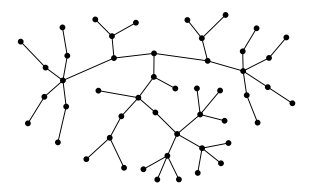
\includegraphics[width=\linewidth]{Tree.png}\\
A tree with 25 leaves.}

\begin{Proposition}
    \label{prop:tree_leaves}
    Let F be a forest with at least one edge (and hence at least two vertices). There are at least two leaves in F.
\end{Proposition}

\textit{Proof.} Let \( \sigma = (v_0, v_1, \ldots, v_k) \) be a path of maximum length in F.
SInce there is at least one edge in F, we have \(\left|\sigma\right| \geq 1\).
The claim is that \( \deg(v_0) = \deg(v_k) = 1 \). Suppose for a contradiction that \( \deg(v_0) \geq 2 \).
So there exists \( u \in V\) such that \( uv_0\) is an edge. If \( u = v_i\) for some \( i \),
then there is a cycle \(v_i, v_0, \ldots, v_i\) contradicting the fact that F is a forest.
Hence for all \( 1 \leq i \leq k \), we have \( u \neq v_i \). But this a path of length \( k+1 \) exists.
This contradicts the maximality of \( \sigma \). \qedsymbol
\marginnote{The intuition is that, a tree should have at least two ends, if not, either there is a cycle or there is
an extending part (a new end) that can be added to the tree.}


\begin{Proposition}[A characterization of trees]
    A graph G = (V,E) is a tree if and only if for all \( u,v \in V \), there
    exist a unique path from \( u \) to \( v \).
\end{Proposition}

\textit{Proof.} First, suppose that G is a tree. Let \( u,v \in V \),
since G is a tree, it is connected, so there must exist some path \(\sigma\) from \( u \) to \( v \).
Now we prove that this path is unique. For a contradiction, let \(\sigma'\) be another path from \( u \) to \( v \).
Both \(\sigma\) and \(\sigma'\) starts at \( u \), but eventually they must diverge.
Let \(v_1\) be the last vertex where \(\sigma\) and \(\sigma'\) have in common (this should be \( u \)).
Eventually they must meet again, since they both end at \( v \). Let \( v_2 \) be the first vertex where they meet again.
Now let \(\sigma''\) be the path obtained by following \(\sigma\) from \( v_1 \) to \( v_2 \), then following
\(\sigma'\) from \( v_2 \) to \( v \). This is a cycle, by choice of \( v_1 \) and \( v_2 \).
But this give us a contradiction, since G is a tree and contains no cycles. 

Now suppose that for all \( u,v \in V \), there exists a unique path from \( u \) to \( v \).
The fact that there exists a path at all between every two vertices immediately implies that G is connected.
It remains to prove that there is no cycle in G. But this is clear, since if
\(\sigma\) is a cycle in G, then picking any two distinct vertices \( u,v \) on \(\sigma\),
we have two distinct paths from \( u \) to \( v \) (clockwise and counterclockwise along \(\sigma\)). \qedsymbol

We can prove another characterization of trees, but we need a lemma first.

\begin{Lemma}[Detour Lemma]
    Let G = (V,E) be a connected graph and let \(\sigma\) be a cycle in \( G \),
    If \( G' \) is the graph obtained by deleting on edge from \(\sigma\), then \( G' \) is still connected.
\end{Lemma}

\begin{Lemma}
    A graph G = (V,E) is a tree if and only if it is connected and \(\left|E\right| = \left|V\right|-1\).
\end{Lemma}

\textit{Proof.} We prove the forward implication by induction on \( n = \left|V\right| \).
Concretely, the statement we shall prove is, for all \(n \geq 1\), for all \(G = (V,E)\) with \(\left|V\right| = n\),
if G is a tree, then \(\left|E\right| = n-1\) and G is connected.

The base case in \( n=1 \), where the only possible graph G is simply a single vertex with no edges.
This is a tree, since it is connected and concains no cycles. We have \(\left|E\right| = 0 = 1-1\).

For the inductive step, let \( n \geq 1 \) and suppose that the statement holds \( n \). Let
\( G = (V,E) \) be a tree with \(\left|V\right| = n+1\). Since \( n\geq 1  \), \( \left|V\right| \geq 2 \),
there are at least two vertices, and the connectedness of G means that there is at least one edge in G.
Hence G is a firest with at least one edge, and by \Cref{prop:tree_leaves}, there are at least two
leaves in G. Pick one of these leaves and call it \( u \). Form a new graph \( G' = (V',E') \) by removing
the leaf \( u \) and the edge incident on it. We have \(\left|V'\right| = n\) and \(\left|E'\right| = \left|E\right|-1\).
The graph \( G' \) is a tree, because for each pair of vertices \( v,w \in V' \), there is a unique path from \( v \) to \( w \)
in G, and this path does not pass through \( u \) (since \( u \) is a leaf). Hence
\[ \left|E\right| = \left|E'\right| + 1 = \left|V'\right| - 1 + 1 = \left|V\right| - 1, \]
where in the second equality we have to used the inductive hypothesis. 

Now assume that G is connected and \(\left|E\right| = \left|V\right| - 1\). We want to show
that G has no cycles. For a contradiction, suppose that \(\sigma\) is a cycle in G. 
Remove an edge from \(\sigma\), by detour lemma, the resulting graph is still connected.
If this graph still has a cycle, remove an edge from it again, and repeat this process until now cycles remain.
This graph G' still has \(\left|V\right|\) vertices, but it has a new edge set \( E' \) with \(\left|E'\right| < \left|E\right|\).
But G' is now a tree, since it contains no cycles but is still connected. So by the
previous paragraph, we have \(\left|E'\right| = \left|V\right| - 1 = \left|E\right|\).
The contradiction completes the proof. \qedsymbol

Now we are ablt the answer the following extremal question: How many edges
can a graph on \( n \) vertices have if it does not contain a cycle (i.e., is a forest)?

\begin{Corollary}
    Let F = (V,E) be a forest, then \(\left|E\right| \leq \left|V\right| - 1\).
\end{Corollary}
\textit{Proof.} Let \( k \geq 1\) denote the number of connected components of F, and
number the connected components as \( C_1, \ldots, C_k \). Join \( C_1 \) to \( C_2 \) by an edge,
then join \( C_2 \) to \( C_3 \) by an edge, and so on. This creates a connected graph G = (V,E')
with \( \left|E'\right| = \left|E\right| + k - 1 \), and G must be a tree, since adding
these edges does not introduce a cycle. By the previous theorem, 
\(\left|E'\right| = \left|V\right| - 1\), so \(\left|E\right| \leq \left|E'\right| = \left|V\right| - 1\). \qedsymbol

\subsection{Eulerian trails and circuits}

Recall that a wak that des not repeat any vertex is called a path. Now we introduce the concept of
\textit{trail}: this is a walk that does not repeat any \textit{edge}.
A walk is called an \textit{Eulerian trail} if it uses every edge of G exactly once, and an
\textit{Eulerian circuit} if it is an Eulerian trail and it is closed.

\marginnote{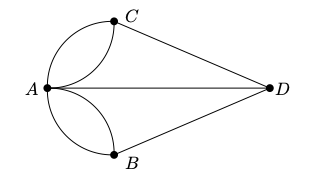
\includegraphics{seven_bridges_of_konigsberg.png}
The graph representing the seven bridges of Konigsberg}


\begin{Theorem}
    Let G = (V,E) be a connected graph with a finite number of vertices and edges, where
    multiple edges between the same pair of vertices are allowed. Then G has an Eulerian circuit
    if and only if every vertex in G has even degree.
\end{Theorem}

\textit{Proof.} Suppose G has an Eulerian circuit \(\sigma = (v_0, v_1, \ldots, v_k)\) where \( v_0=v_n \)
For each \( v_i \neq v_0 \), each visit uses two edges, one edge to enter \( v_i \) and one edge to leave \( v_i \).
So \( \deg(v_i) \) is even for all \( 0\leq i < n \). For \( v_0 = n \), there is one edge that leaves it at the
beginning, two edges for each visit during the circuit, and then one returning to it at the end. 
So \( \deg(v_0) \) is even as well.

We prove the reverse implication by induction on \( m = \left|E\right| \). That is,
we prove that for all integers \( m \geq 0 \), if G = (V,E) with \(\left|E\right| = m\) and all
vertices in G have even degree, then G has an Eulerian circuit.

For the base case \( m = 0 \), the graph G is a single vertex with no edges, and it has an Eulerian circuit.

Now let \( m \geq 1 \) and suppose the statement holds for all integers less than or equal to \( m \).
Let G = (V,E) with \(\left|E\right| = m +1 \). Since there is at least one edge in G,
G cannot be a tree. This is because every tree with at least one edge contains at least two leaves,
and leaves have (odd) degree 1. Let \(\sigma\) be a cycle in G
and form a new graph G' = (V,E') by deleting every edge in \(\sigma\). This graph
may no longer be connected, but since we remove a cycle, every vertex in G' either has the
same degree as in G, or degree two less than in G. So all vertices in G' have even degree as well.
Let k be the number of connected components of G'; number them as \( H_1, \ldots, H_k \).
\marginnote{\textbf{Process of building an Eulerian circuit in G:}
\begin{itemize}
    \item Start at any vertex \( \sigma \)
    \item Follow \( \sigma \)
    \item Each time we reach a vertex of a connected component \( H_i \) of G' for
    the first time, follow its Eulerian circuit. 
    \textit{(We know that each connected component has an Eulerian circuit by the inductive hypothesis.)}
    \item Once we return to the beginning of the Eulerian circuit, continue along \( \sigma \).
    \item Repeat this process until we return to the vertex of \( \sigma \) we started at.
\end{itemize}}
Each has at most \( m \) edges, so by the inductive hypothesis, each has an Eulerian circuit.

We build an Eulerian circuit in G using the process to the right.
Eventually, this gives us an Eulerian circuit in G. \qedsymbol

\begin{Theorem}
    Let G = (V,E) be a connected graph (with multiple edges allowed). Then G contains an Eulerian trail
    that isn't an Eulerian circuit if and only if exactly two vertices of G have odd degree.
\end{Theorem}

\textit{Proof.} Suppose that G contains an Eulerian trail \( \sigma = (v_0, v_1, \ldots, v_k) \) in which \( v_0 \neq v_k \).
By a similar reasoning to the first paragraph of the previous proof, every vertex in the walk has even degree, except both \( v_0 \) and \( v_k \)
must have odd degree, since starting at \( v_0 \) we must leave for the first time via an edge, and at the end we enter
\( v_k \) one last time without exiting.

Now assume that G contains exactly two odd-degree vertices. By the previous theorem, there does not exist an
Eulerian circuit in G. Let \( u \) and \( v \) be the two odd-degree vertices. Add a new edge \( uv \), even if there was
already an edge between \( u \) and \( v \) before. We get G' in which every vertex has even degree.
So G' must have an Eulerian circuit \( \sigma' \). It contains the edge \( uv \), but we can remove it
to get an Eulerian trail in G. \qedsymbol

\subsection{Planar graphs}

A graph G is called \textit{planar} if it can be drawn in the plane without any edges crossing.
If we can, such a drawing is called a \textit{planar embedding} of G.
\marginnote{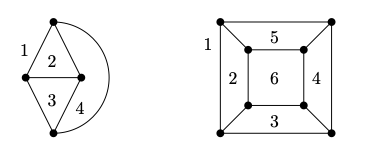
\includegraphics{planar_embeddings.png}
Planar embeddings of \( K_4 \) and \( Q_{3}\)}

Planarity is a property that passes down to subgraphs.

\begin{Proposition}
    \label{prop:planar_subgraph}
    If G is planar then any subgraph H of G is also planar.
\end{Proposition}

\textit{Proof.} If G is drawn in the plane without edges crossing, and we erase some
edges and vertices to create a drawing of H, we cannot introduce any edge crossings along the way. \qedsymbol

A planar embedding of a graph determins regions, or \textit{faces} bounded by edges, 
including on region outside the graph.
We define the \textit{Euler characteristic} of a planar embedding of G to be the quantity
\[\chi = \left|V\right| - \left|E\right| + f,\]
where \( f \) is the number of faces in the embedding.

From the figure above, we notice that both \( K_4 \) and \( Q_3 \) have \(\chi = 2\), this is not just a coincidence.

\begin{Theorem}[Euler's formula]
    \label{thm:euler_formula}
    Let G = (V,E) be a connected planar graph, let \(f\) be the number of faces in a planar embedding of G.
    Then \( \left|V\right| - \left|E\right| + f = 2 \).
\end{Theorem}

To prove this, we need the following theorem.

\begin{Theorem}[Jordan curve theorem]
    Every closed curve in the plane \(\mathbb{R}^2 \) that does not intersect itself divides the plane into two regions.
\end{Theorem}

\textit{Proof of \Cref{thm:euler_formula}.} We proceed by induction on \( m = \left|E\right| \).
In the case that \( m=0 \), G can only be a single vertex, in which we have \( \chi = 1-0+1 = 2 \).

Now let \( m \geq 0 \) and assume that the theorem holds for all natural numbers at most m.
Let G = (V,E) be a connected planar graph with \(\left|E\right| = m+1\).
Draw G in the plane and let f be the number of faces in the embedding.
There are two cases, according to whether G is a tree or not.
If G is a tree, then \( f =1\) since G has no cycles. But we also have \(\left|E\right| = \left|V\right| - 1\), so
\[\chi = \left|V\right| - \left|E\right| + f = \left|V\right| - \left|V\right| + 1 + 1 = 2.\]
If G is not a tree, then G has a cycle, call it \(\sigma\). Form G' by removing exactly one edge \( e \) from \(\sigma\), so
\[\left|E'\right| = \left|E\right| - 1 = m + 1 - 1 = m.\]
By the detour lemma, G' is still connected, and it is planar, since removing an edge doesn't introduce any crossings.
By the inductive hypothesis, the Euler characteristic \( \chi' \) of G' satisfies
\[\chi' = \left|V\right| - \left|E'\right| + f' = 2,\]
where \( f' \) is the number of faces in a planar embedding of G'.
Returning to the drawing of G, the cycle \(\sigma\) is closed curve without intersections in the plane, so it divides
the plane into two regions (each of which may have multiple faces within them).
In particular, the removed edge \( e \) forms a border between two distinct daces, and in G',
these two faces combine into one face. Hence \( f = f' + 1 \).
Putting everything together, we calculate the Euler characteristic of G satisfies
\[\chi = \left|V\right| - \left|E\right| + f = \left|V\right| - (\left|E'\right|+1) + (f'+1) + 1 = 2.\quad \qedsymbol\]

Euler's formula tells us that the number of faces in any drawing of G depends entirely on
the number of vertices and edges in G. We can use this information to give conditions for a graph to be non-planar.

\begin{Theorem}
    \label{thm:nonplanar_bound}
    Let G = (V,E) be a connected planar graph with \( \left|V\right| \geq 5 \). The
    \[\left|E\right| \leq 3\left|V\right| - 6.\]
    Under the further assumption that G contains no triangles, we have a better bound
    \[\left|E\right| \leq 2\left|V\right| - 4.\]
\end{Theorem}

\textit{Proof.} The proof is by double counting. Let R be the set
of all regions into which G divides the plane, so that \( \left|R\right| =f\),
the number of faces. Consider the set
\[S = \{(e,r) \subset E \times R: \text{the edge e touches the region r}\}.\]
We will count \( \left|S\right| \) in two ways. First off, each edge \( e\in E \) touches
at most two regions, so \( \left|S\right| \leq 2\left|E\right| \).
On the other hand, every region is bounded by a cycle, and\
a cycle has at least three edges, so each region \( r \in R \) touches
at least 3 edges. In other words, \( \left|S\right| \geq 3f \).
Chaining these into two inequalities, we have
\[3f \leq \left|S\right| \leq 2\left|E\right|.\]
But by Euler's formula, we have \( \left|V\right| - \left|E\right| + f = 2 \), so
\(f = 2 + \left|E\right| - \left|V\right|\), and substituting this
above, we get
\[3(2 + \left|E\right| - \left|V\right|) \leq 2\left|E\right|.\]
Distributing and rearranging terms yields the desired
inequality \( \left|E\right| \leq 3\left|V\right| - 6 \).

If we have the further assumption that there are no triangles in G,
then every region must touch at least 4 edges, allowing us
to conclude the stronger inequality \( 4f \leq 2 \left|E\right| \).
Then we proceed as above to get
\[ 4(2 - \left|V\right| + \left|E\right|) \leq 2\left|E\right|,\]
which can be manipulated to get
\( \left|E\right| \leq 2\left|V\right| - 4 \). \qedsymbol

The condition that \( \left|V\right| \geq 5 \) is a complete non-issue, since a graph with
fewer than 5 vertices is a subgraph of \( K_4 \), and we can apply \Cref{prop:planar_subgraph},
since we already know that \( K_4 \) is planar. As a corollary of the (contrapositive of the) 
previous theorem, we can give two important examples of nonplanar graphs.

\begin{Corollary}
    The complete graph \( K_5 \) and the complete bipartite graph \( K_{3,3} \) are nonplanar.
\end{Corollary}

\textit{Proof.} If \((V,E) = K_5\) we have \( \left|V\right| = 5 \) so \( 3 \left|V\right| - 6 = 9 \), but
\( \left|E\right| = 10 \). So by the contrapositive of the previous theorem, \( K_5 \) is nonplanar.

The graph \( K_{3,3} \) does not contain any triangles, so if it were planar, then the stronger bound
\( \left|E\right| \leq 2\left|V\right| - 4 \) must hold. But in \((V,E) = K_{3,3}\), we have
\( \left|V\right| = 6 \) and \( 2\left|V\right| - 4 = 8 \), but \( \left|E\right| = 9 \). So \( K_{3,3} \) is nonplanar. \qedsymbol

This corollary, combined with the contrapositive of \Cref{prop:planar_subgraph}, shows that \( K_n \) is nonplanar
for all \( n \geq 5 \), and that \( K_{m,n} \) is nonplanar for all \( m,n \geq 3 \). More generally, any graph
that contains \( K_5 \) or \( K_{3,3} \) as a subgraph is nonplanar.

\marginnote{
\begin{center}
    \label{fig:nonplanar_graph}
    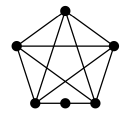
\includegraphics[width=0.4\linewidth]{k_5_w_extra_vertex.png}\\
\end{center}
The graph \( K_5 \) with an extra vertex subdividing an edge.}
However, subgraphs are not exactly the right notion to be considering when talking about planarity.
To see why, consider the graph to the right.

It is nonplanar, since if it had a planar embedding, then by contracting on of the edges incident on the vertex,
and bending other edges accordingly, we would obtain a planar embedding of \( K_5 \). On the other hand,
this graph does not contain \( K_5 \) as a subgraph. We thus introduce the following notion.

We say that a graph \( H \) is a \textit{graph minor} of a graph \( G \) if \( H \) can be obtained from G repeatedly by either
one of the following operations to the right.
\marginnote{
    \begin{itemize}
        \item deleting an edge;
        \item deleting a vertex; or
        \item contracting an edge \( uv \) by removing it and merging
        \( u \) and \( v \) into a single vertex (and also combining any resulting multiple edges into a single edge).
    \end{itemize}
}

Any number of the first two operations simply creates a subgraph. It is the contraction operation that produces interesting
examples of graph minors. It is easy to see pictorially that contracting edges preserves planarity,
so any graph minor of a planar graph is planar. We can use this to show, for instance, that the Petersen graph,
depicted to the right, is nonplanar. Since by contracting each of the five edges connecting the inner star pentagram
to the other pentagon, we obtain a \( K_{5} \). (Note that \Cref{thm:nonplanar_bound} does not apply to the Petersen graph.)

Not only all graphs that have \( K_5 \) and \( K_{3,3} \) as minors are nonplanar, it turns out that
there are the only nonplanar graphs.

\begin{Theorem}[Wagner's theorem]
    A graph G is nonplanar if and only if either \(K_5\) or \(K_{3,3}\) is a minor of G.
\end{Theorem}

It deals with the notion of a \textit{subdivision} of a graph G, subdividing an edge into two edges each time. 
(We have shown an example of a subdivision of \( K_5 \) )

\begin{Theorem}[Kuratowski's theorem]
    A graph \(G\) is nonplanar if and only if it contains a subdivision of either \(K_5\) or \(K_{3,3}\) as a subgraph.
\end{Theorem}

It is easy to see that if H is a subdivision of G, then G is a minor of H,
since we can reobtain G by contracting all the edges created by the subdivision
operations. So the two theorems above are certainly very closely related, though
it is not immediately obvious if one should imply the other. The truth is that
they are equivalent, because it can be shown that any graph with either \( K_5 \) or
\( K_{3,3} \) as a minor also has a subgraph that is a subdivision of one of them.

\section{Combinatorics}

\subsection{Counting}

\begin{Theorem}[Principle of inclusion and exclusion]
    \label{thm:inclusion_exclusion}
    Let \( n\geq 2 \) be an integer and let \( A_1, \ldots , A_n \)
    be finite sets. Then
    \[\left|\bigcup_{i}^{n}A_i\right| =\sum_{k=1}^{n}(-1)^{k+1}\left(\sum_{1\leq i_1 < \ldots < i_k \leq n}\left|\bigcap_{j=1}^{k}A_{i_j}\right|\right).\]
\end{Theorem}

\begin{Theorem}[Binomial theorem]
    For all \( x,y\in \mathbb{R} \) and positive integers \( n \),
    \[(x+y)^n = \sum_{k=0}^{n}\binom{n}{k}x^{n-k}y^k.\]
\end{Theorem}

\textit{Proof.} Expanding the left-hand side, we get
\[(x+y)^n = \underbrace{(x+y)(x+y)\cdots(x+y)}_{n \text{ times}}.\]
We see that there will be \( 2^n \) different terms after repeatedly using the
distributive property. Each term will be a product of \( x \) to some power and
\( y \) to some power, where the powers add up to n. In other words, each term
will be of the form \( x^{n-k}y^k \) for some \( k \) between 0 and \( n \).
The number of times that the term \( x^{n-k}y^k \) appears is the number of ways
to choose \( k \) of the \( n \) factors to be \( y \), which is \( \binom{n}{k} \).
This gives exactly the right-hand side of the equation. \qedsymbol

\textit{Proof of \Cref{thm:inclusion_exclusion}.}
Let \( n \geq 2 \) and let \( A_1, A_2, \ldots , A_n \) be finite sets. Recall that
the identity we want to prove is 
\[\left|\bigcup_{i=1}^{n}A_i\right| = \sum_{k=1}^{n}(-1)^{k+1}\left(\sum_{1\leq i_1 < \ldots < i_k \leq n}\left|\bigcap_{j=1}^{k}A_{i_j}\right|\right).\]
Let \( x \) be an element that belongs to the union \( \bigcup_{i=1}^{n} A_i\). Clearly, this contributes
1 to the left-hand side, so we must show that it contributes exactly 1 to the right-hand side as well.
We know that \( x \) is a member of at least one of \( A_i \); let \( s\geq 1 \)
be the number of the sets \( A_i \) that contain \( x \).

Each time \( x \) is a member of some \( A_i \), it contributes +1 to the right-hand side.
This happens \( \binom{s}{1} \) times. Each time it is a member of \( A_i \) and \( A_j \) for some \( i < j \),
\( x \) contributes -1 to the right-hand side; this happens \( \binom{s}{2} \) times. generally,
if \( x \) is a member of \( A_1 \cap A_2 \cap \ldots \cap A_r \), it contributes +1 if \( r \) is odd
and -1 if \( r \) is even, and this term is repeated \( \binom{s}{r} \). 
So the total contribution of \( x \) to the right-hand side is
\[\binom{s}{1} - \binom{s}{2} + \binom{s}{3} - \ldots + (-1)^{s+1}\binom{s}{s}\]
By the binomial theorem, 
\[ 0 = (1-1)^s = \binom{s}{0} - \binom{s}{1} + \binom{s}{2} - \ldots + (-1)^s\binom{s}{s}.\]
We know that \( \binom{s}{0} = 1 \), so by rearranging the terms, we get
\[\binom{s}{1} - \binom{s}{2} + \binom{s}{3} - \ldots + (-1)^{s+1}\binom{s}{s} =\binom{s}{0} = 1.\]
This means that the contribution of \( x \) to the right-hand side is 1, as desired. 
The proof is finished since \( x \) is arbitrary.\qedsymbol

\begin{Example}
Let \( X = \{1,2,\ldots,100\} \) and we want to count the number of \( n \in \mathbb{X} \)
with \( \gcd(n,30) = 1\). 
\end{Example}
To accomplish this, it turns out to be easier to count the number of \( n \in X \) with \( \gcd(n,30) \geq 2 \)
(and then we must subtract this number from \( \left|X\right| = 100 \)). For
any positive integer \( r \) let
\[ A_r = \{n \in X: r|n\}.\]
Since \( 30 = 2 \cdot 3 \cdot 5 \), an integer \( n \) has \( \gcd(n,30) \geq 2 \) if and only if
\( n \in A_2, n \in A_3, \text{ or } n \in A_5 \). By the principle of inclusion and exclusion,
\[\left|A_2 \cup A_3 \cup A_5\right| = \left|A_2\right| + \left|A_3\right| + \left|A_5\right| - \left|A_2 \cap A_3\right| - 
\left|A_2 \cap A_5\right| - \left|A_3 \cap A_5\right| + \left|A_2 \cap A_3 \cap A_5\right|.\]

The number of even integers in \( X \) is \( \left|A_2\right| = 50 \), similarly the number of multiples of 3 is 
\( \left|A_3\right| = \lfloor100 \slash 3 \rfloor= 33 \). In general, \( \left|A_r\right| = \lfloor 100 \slash 4 \rfloor \).
Furthermore, since \( \gcd(2,3) = 1 \), the intersection \( A_2 \cap A_3 \) is simply \( A_6 \),
and by analogous reasoning, we see that
\begin{align*}
    \left|A_2 \cup A_3 \cup A_5\right| &= \left|A_2\right| + \left|A_3\right| + \left|A_5\right| - \left|A_6\right| 
    - \left|A_{10}\right| - \left|A_{15}\right| + \left|A_{30}\right|\\
    &= \lfloor\frac{100}{2}\rfloor + \lfloor\frac{100}{3}\rfloor + \lfloor\frac{100}{5}\rfloor - \lfloor\frac{100}{6}\rfloor
    - \lfloor\frac{100}{10}\rfloor - \lfloor\frac{100}{15}\rfloor + \lfloor\frac{100}{30}\rfloor\\
    &= 50 + 33 + 20 - 16 - 10 - 6 + 3 \\
    &= 74.
\end{align*}
We conclude that the number of \( n \in X \) with \( \gcd(n,30) = 1 \) is \( 100 - 74 = 26 \).

\subsection{Permutations and combinations}

\begin{Proposition}
    Let \( n \geq 0 \) be an integer. Then
    \[ \sum_{k=0}^{n}\binom{n}{k}^2 = \binom{2n}{n}.\]
\end{Proposition}

\textit{Proof.} Let X be set of size 2n. The right-hand side counts the number of subsets of X of size n.
We count this in a different way. Let A and B be such the \( \left|A\right| = \left|B\right| = n \),
and \( A\cup B = X \) (so we must have \( A \cap B = \emptyset \)). Then
choosing a subset of X is the same as choosing \( k \) elements of A, where \( 0 \leq k \leq n \),
and then choosing the remaining \( n-k \) elements from B. In other words,
\[\binom{2n}{n} = \sum_{k=0}^{n}\binom{n}{k}\binom{n}{n-k} = \sum_{k=0}^{n}\binom{n}{k}^2.\]
\hfill \qedsymbol

Now let's explore more identities involving binomial coefficients.
\marginnote{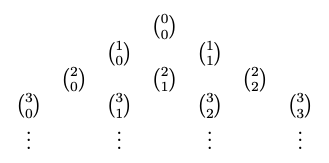
\includegraphics{Pascel's_triangle_1.png} \\
Laying out the binomial coefficients in the triangle.
}

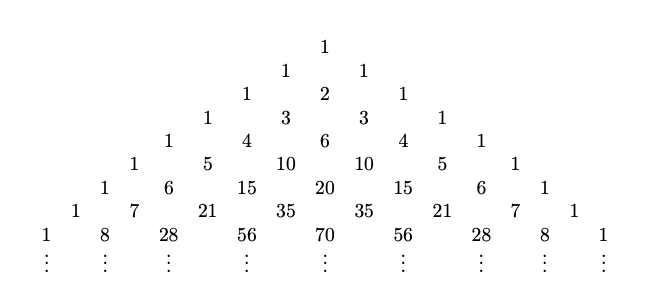
\includegraphics{Pascel's_triangle_2.png}\\
\label{fig:pascal_triangle}
\begin{center}
    Pascal's triangle
\end{center}

This triangle can easily be drawn by hand by writing 1s along its boundary and filling in the interior
by adding the two numbers above each cell. Now we shall prove this observation.

\begin{Proposition}[Pascal's identity]
    Let \( n \geq 0 \) and \( k\geq 1 \) be integers. Then
    \[\binom{n}{k} = \binom{n-1}{k} + \binom{n-1}{k-1}.\]
\end{Proposition}
\marginnote{The only number that appears infinitely many times is 1, since any \( n \in Z \)
can only appear in the first n + 1 rows of the triangle.\\
A fun conjecture to think about is the Singmaster's conjecture, but whether the statement is true is still 
a open problem.}

\textit{Proof.} Set \( X = \{1,2,\ldots,n\} \). We count the number of sets \( Y \subseteq X  \) there 
are of size \( k  \). Either \( 1 \in Y  \) or \( 1 \notin Y  \). If \( 1 \notin Y  \),
then there are \( \binom{n-1}{k} \) possibilities for what \( Y \) can be. If \( 1 \in Y  \),
then there are still \( k-1 \) elements to choose from \( n-1 \) elements, so there are \( \binom{n-1}{k-1} \) possibilities for what \( Y \) can be. 
Hence the right-hand side counts the number of sets \( Y \subseteq X \) of size \( k \). But
this is exactly what the left-hand side counts as well. \hfill \qedsymbol

\textit{Another proof of \Cref{prop:even_odd_cardinality}} We re-establish the notation of the
proposition statement. Let X be a finite nonempty set, let E be the set of subsets of X with even cardinality, and let O
bet the set of subsets with odd cardinality. By the binomial theorem with \( x = -1, y = 1 \), we have
\begin{align*}
0 &= (-1+1)^n =  \sum_{k=0}^{n}\binom{n}{k}(-1)^k1^{n-k}\\
    &= \binom{n}{0} - \binom{n}{1} + \binom{n}{2} - \ldots + (-1)^n\binom{n}{n}\\
\end{align*}
Hence 
\[\binom{n}{0} + \binom{n}{2} + \ldots + \binom{n}{n} = \binom{n}{1} + \binom{n}{3} + \ldots + \binom{n}{n-1}.\]
but the left-hand side is just \( \left|E\right| \) and the right-hand side is \( \left|O\right| \). \hfill \qedsymbol

\begin{Proposition}
    For all \( n \in \mathbb{N} \),
    \[\sum_{k=0}^{n}\binom{n}{k} = 2^n.\]
\end{Proposition}

\textit{Proof.} By the binomial theorem with \( x = y = 1 \), we have
\[2^n = (1+1)^n = \sum_{k=0}^{n}\binom{n}{k}1^k 1^{n-k}= \sum_{k=0}^{n}\binom{n}{k}.\]
The proposition can also be proven by noting that the left-hand side counts the number of subsets of
\( \{1,2,\ldots,n \} \) of size 0, plus the subsets of size 1, and so on up to all subsets of size n.
But adding up all these numbers gives the number of all subsets of \( \{1,2,\ldots,n \} \), which is \( 2^n \). \hfill \qedsymbol 

\begin{Theorem}[Freshman's dream]
    Let p be a prime number and let \( x,y \in \mathbb{Z}\).
    Then 
    \[(x+y)^p=x^p + y^p \pmod{p}.\]
\end{Theorem}

\textit{Proof.} By the binomial theorem, we have
\[(x+y)^p = \sum_{k=0}^{p}\binom{p}{k}x^{k}y^{p-k} = x^{p} + y^p + \sum_{k=1}^{p-1}\binom{p}{k}x^{k}y^{p-k}.\]
Taking this equation modulo p, we are done if we can show that for all \( 1 \leq k \leq p-1 \),
\[\binom{p}{k} \equiv 0 \pmod{p}.\]
Let \( 1 \leq k \leq p-1 \) and expand the binomial coefficient:
\[\binom{p}{k} = \frac{p!}{k!(p-k)!}.\]
Multiplying both side by \( k!(p-k)!\), we get
\[k!(p-k)!\binom{p}{k} = p! = p(p-1)!.\]
This is an integer and the right-hand side is a multiple of \( p \), so the left-hand side is as well.
Then since \( p \) devides the product \( k!(p-k)! \), either \( p \) divides \( k!(p-k)!\) or it 
divides \( \binom{p}{k} \). But the former is not possible, since
\[k!(p-k)! = k(k-1)\cdots 2\cdot 1 \cdot (p-k)(p-k-1)\cdots 2\cdot 1,\]
and all of the factors on the right-hand side are positive integers less than \( p \).
Hence \( p \) can not divide any of them, and not divide \( k!(p-k)!\),
 so it must divide \( \binom{p}{k} \). \hfill \qedsymbol


\subsection{Recurrence}
\begin{Proposition}
    Suppose that \( (a_n)\) is a sequence with \( a_0=c \)
    for some constant \( c \in \mathbb{R} \) and, for all \( n \geq 0 \),
    \( a_n=b\cdot a_{n-1} \) for some \( b \in \mathbb{R} \). Then for all \( n \geq 0 \),
    we have
    \[ a_n = c\cdot b^n.\]
\end{Proposition}

In general, we will consider recurrences of the form
\[ a_n = f_1(n)a_{n-1} + f_2(n)a_{n-2} + \ldots + f_k(n)a_{n-k} + g(n),\]
where \( f_1, \ldots, f_k,g: \mathbb{N} \to \mathbb{R} \) are functions, and \( k\geq 1 \) is an integer.

These recurrences are said to be \textit{linear of degree k}. If \( g(n) = 0 \),
the recurrence is said to be \textit{homogeneous}; otherwise, it is \textit{non-homogeneous}.

For \textit{non-homogeneous} recurrences, the same recurrence without the \( g(n) \) term 
is called the \textit{associated homogeneous recurrence}. If, for all \( 1\leq i \leq k \), the
function \( f_i \) is a constant function, then the recurrence is said to have \textit{constant coefficients}.

A sequence \( (p_n) \) that satisfies the recurrence is called a \textit{particular solution}.
A \textit{general solution} is a formula describing all possible solution using some parameters.
If we specify values for the first few terms, these are call \textit{initial conditions} for the recurrence.

\begin{Theorem}
    Consider the non-homogeneous recurrence
    \[ a_n = f(n)a_{n-1} + g(n),\]
    where \( f,g: \mathbb{N} \to \mathbb{R} \). If \( (p_n) \) is 
    any particular solution to the recurrence and \( (h_n) \) is a
    general solution to the associated homogenous recurrence, i.e.,
    \[ h_n = f(n)h_{n-1},\]
    for all \( n \geq 1 \), then the general solution
    for recurrence is
    \[ a_n = h_n + p_n.\]
\end{Theorem}

\begin{Theorem}
    Consider the recurrence
    \[a_n = f_1(n)a_{n-1} + f_2(n)a_{n-2} + \dots +
    f_k(n)a_{n-k} + g(n),\]
    for some \( k \geq 1 \) and \( f_1, \ldots, f_k, g: \mathbb{N} \to \mathbb{R} \).
    If \( (p_n) \) is any particular solution to the recurrence
    and \( (h_n) \) is a general solution to the
    associated homogeneous recurrence, i.e.,
    \[ h_n = f_1(n)h_{n-1} + f_2(n)h_{n-2} + \dots + f_k(n)h_{n-k},\]
    for all \( n \geq 1 \), then the general solution for the recurrence is
    given by \( a_n = h_n + p_n \).
\end{Theorem}

\begin{Theorem}
    Consider the recurrence given by
    \[ a_n = c_1a_{n-1}.\]
    If the characteristic polynomial of this recurrence has two
    distinct roots \( r_1 \) and \( r_2 \), then the general solution
    of the recurrence is
    \[ a_n = \alpha_1r_1^n + \alpha_2r_2^n.\]
    Supposing we know the initial conditions \( a_0 \) and \( a_1 \),
    we have the identities
    \[\alpha_1 = \frac{a_1 - r_2a_0}{r_1 - r_2} 
    \quad \text{and} \quad \alpha_2 = \frac{r_1a_0 - a_1}{r_1 - r_2}.\]
\end{Theorem}

\begin{Theorem}
    Let \( k \geq 2 \) be an integer and consider the recurrence given by
    \[ a_n = c_1a_{n-1} + c_2a_{n-2} + \dots + c_ka_{n-k}.\]
    If the characteristic polynomial of this recurrence has \( k \) pairwise distinct roots
    \( r_1, \ldots, r_k \), then the general solution of the recurrence is
    \[ a_n = \alpha_1r_1^n + \alpha_2r_2^n + \dots + \alpha_kr_k^n.\]
\end{Theorem}

\begin{Theorem}
    Consider the homogeneous recurrence
    \[ a_n = c_1a_{n-1} + c_2a_{n-2}.\]
    If the characteristic polynomial of this recurrence has 
    a repeated root \( r \), then the general solution of
    the recurrence is
    \[ a_n = \alpha_1r^n + \alpha_2nr^n.\]
    Suppose we know the initial conditions \( a_0 \) and \( a_1 \),
    then we have the identities
    \[\alpha_1 = a_0 \quad \text{and} \quad \alpha_2 = \frac{a_1 - a_0r}{r}.\]
\end{Theorem}

% end of main text

\makeatletter
  \renewcommand{\section}{\@startsection{section}%
    {3}{0.8em}{-3ex \@plus -1ex \@minus -.2ex}%
    {1.5ex \@plus .2ex}
    {\hspace*{-5.5em}\fcolorbox{Periwinkle}{Periwinkle}{\parbox[c][1.0ex][b]{4em}{\phantom{space}}}
    \normalfont\Large\itshape\color{blue}}}
\makeatother

\bibliography{marginnotes}
\bibliographystyle{plainnat}

\end{document}
